\chapter{Plankbeek catchment}\label{ch:appendixB}
\chaptermark{Appendix B}

\begin{figure}[tbhp]
	\centering
		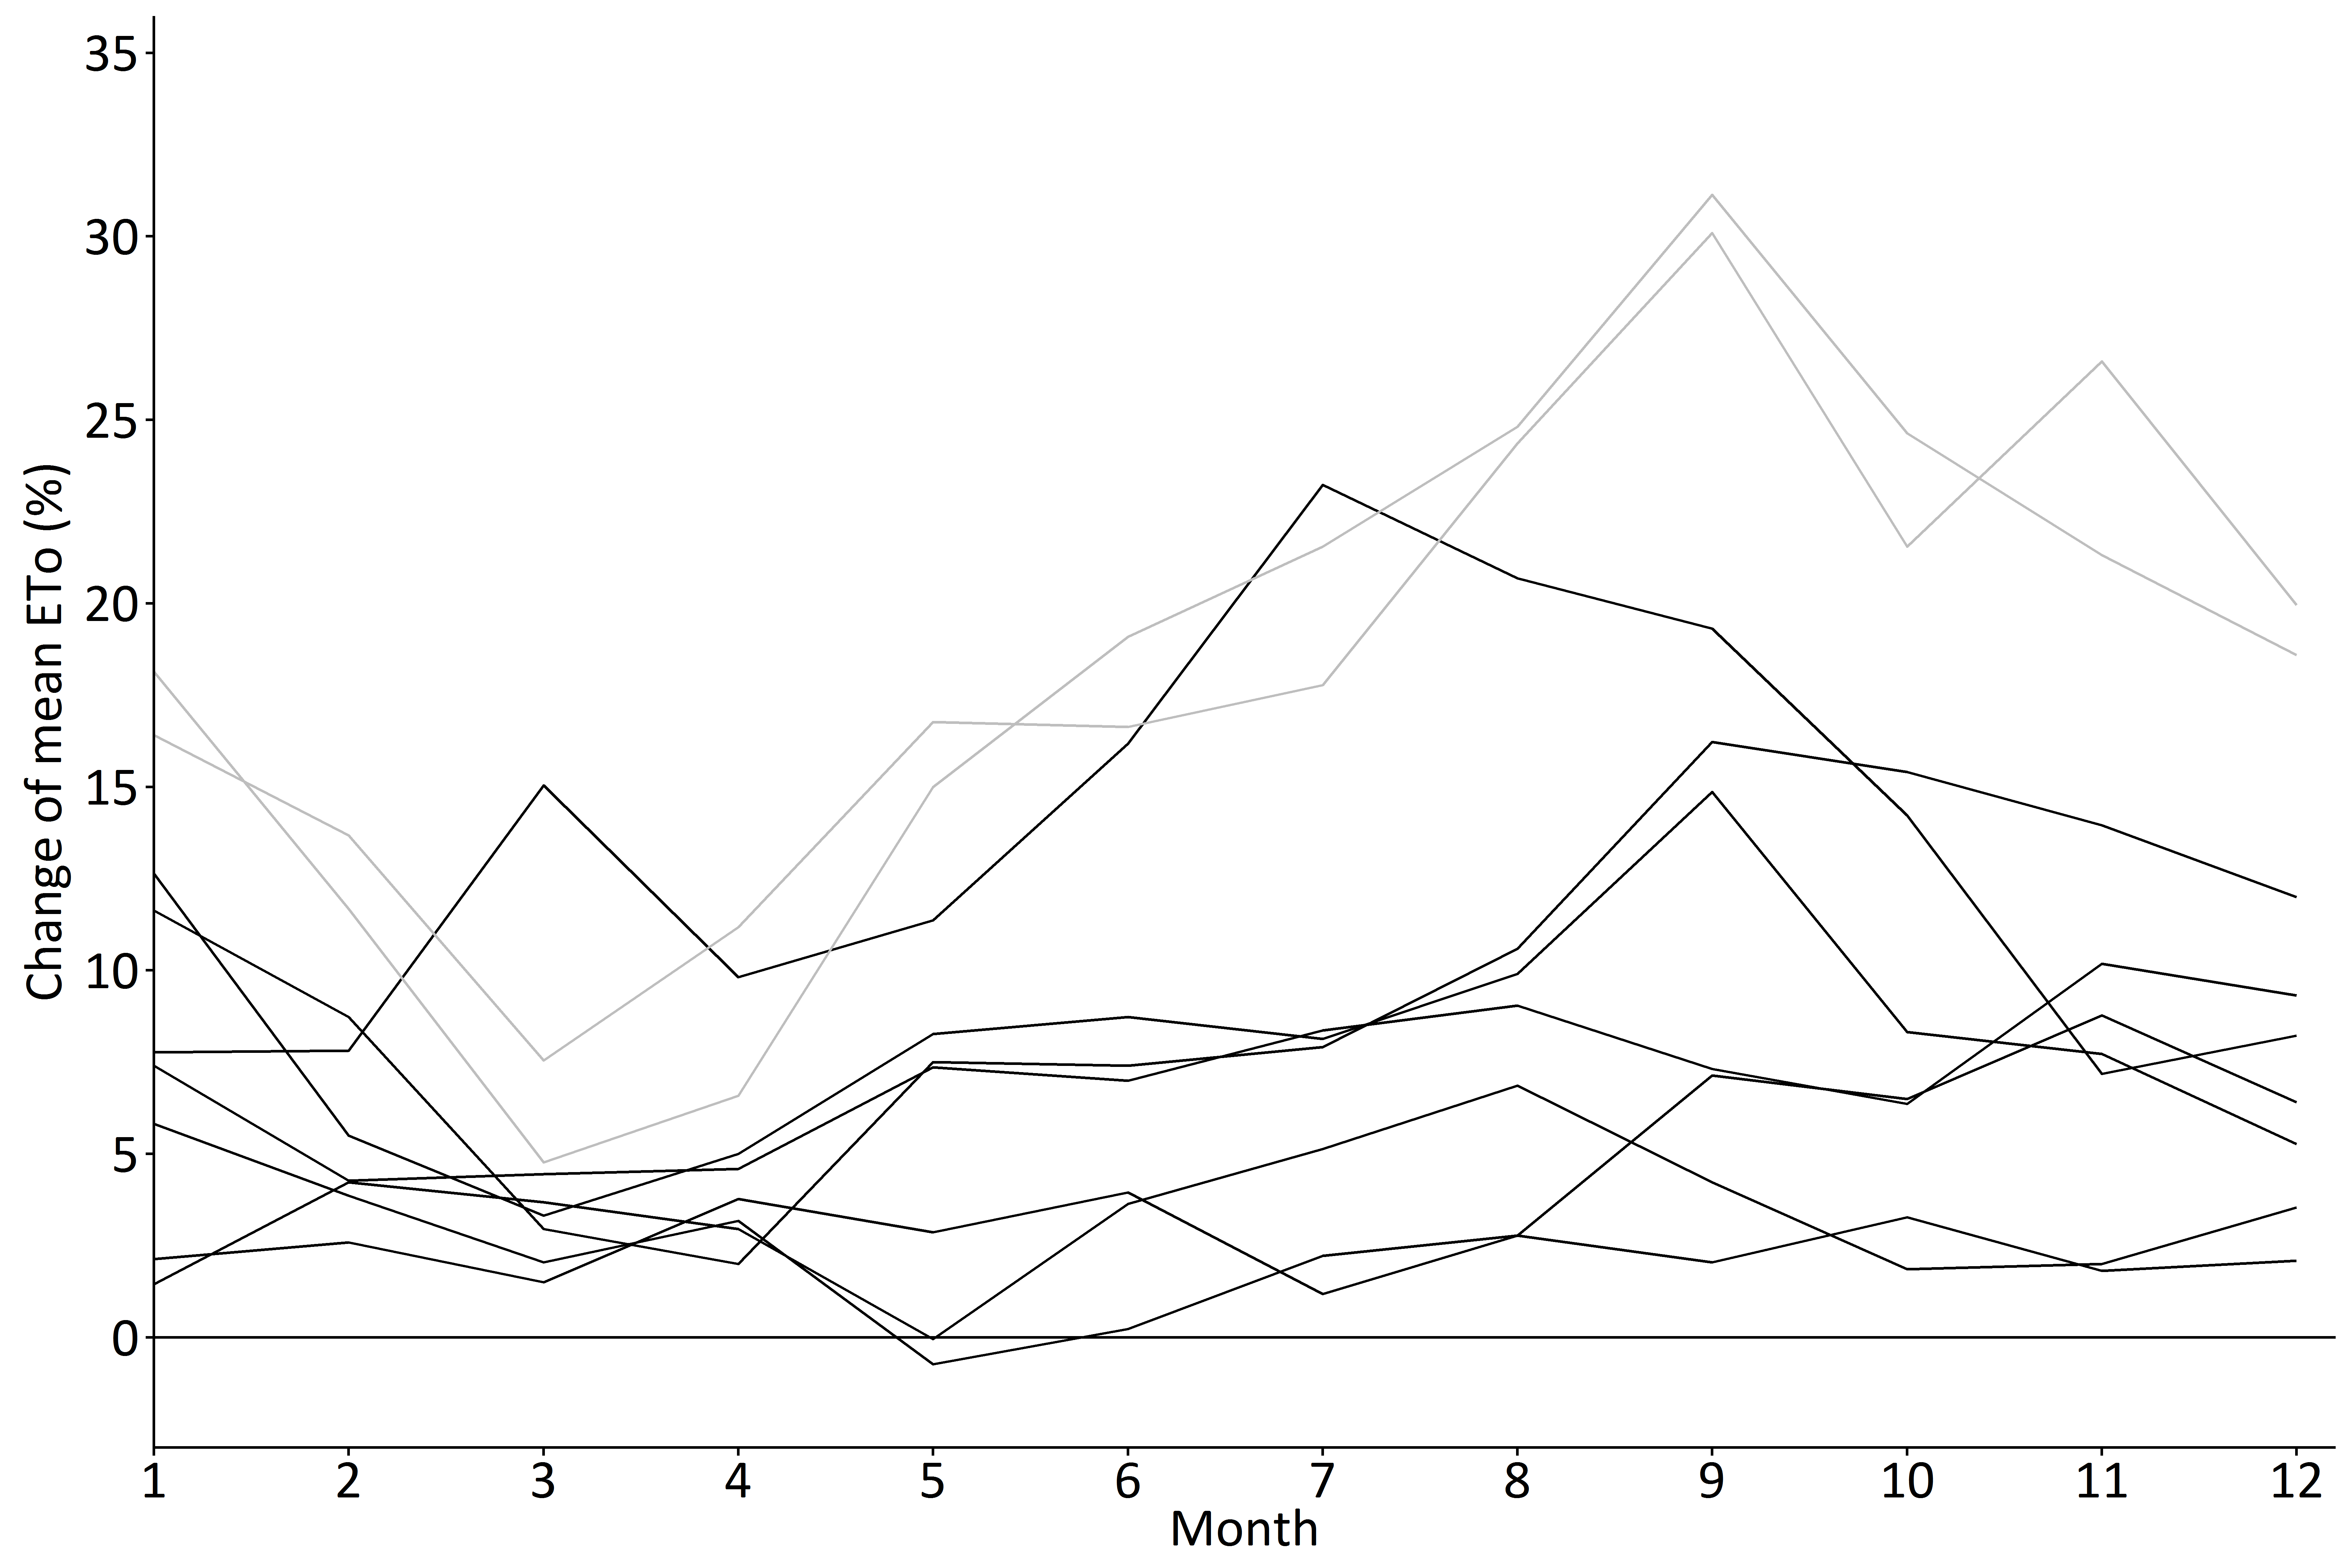
\includegraphics[width=\textwidth]{PerturbETo.png}
	\caption{Relative change of mean reference evapotranspiration (\ETo) in future climatic conditions (2050) as compared to historical conditions (2000) for RCP 8.5. Black lines present the climate signals selected for the climate model ensemble, while grey lines present the additional climate signals that were used to define the synthesized scenarios. A positive value represents an increase of \ETo, while a negative represents a decrease of \ETo.}
	\label{fig:AppB_PerturbETo}
\end{figure} 

\begin{figure}[tbhp]
	\centering
		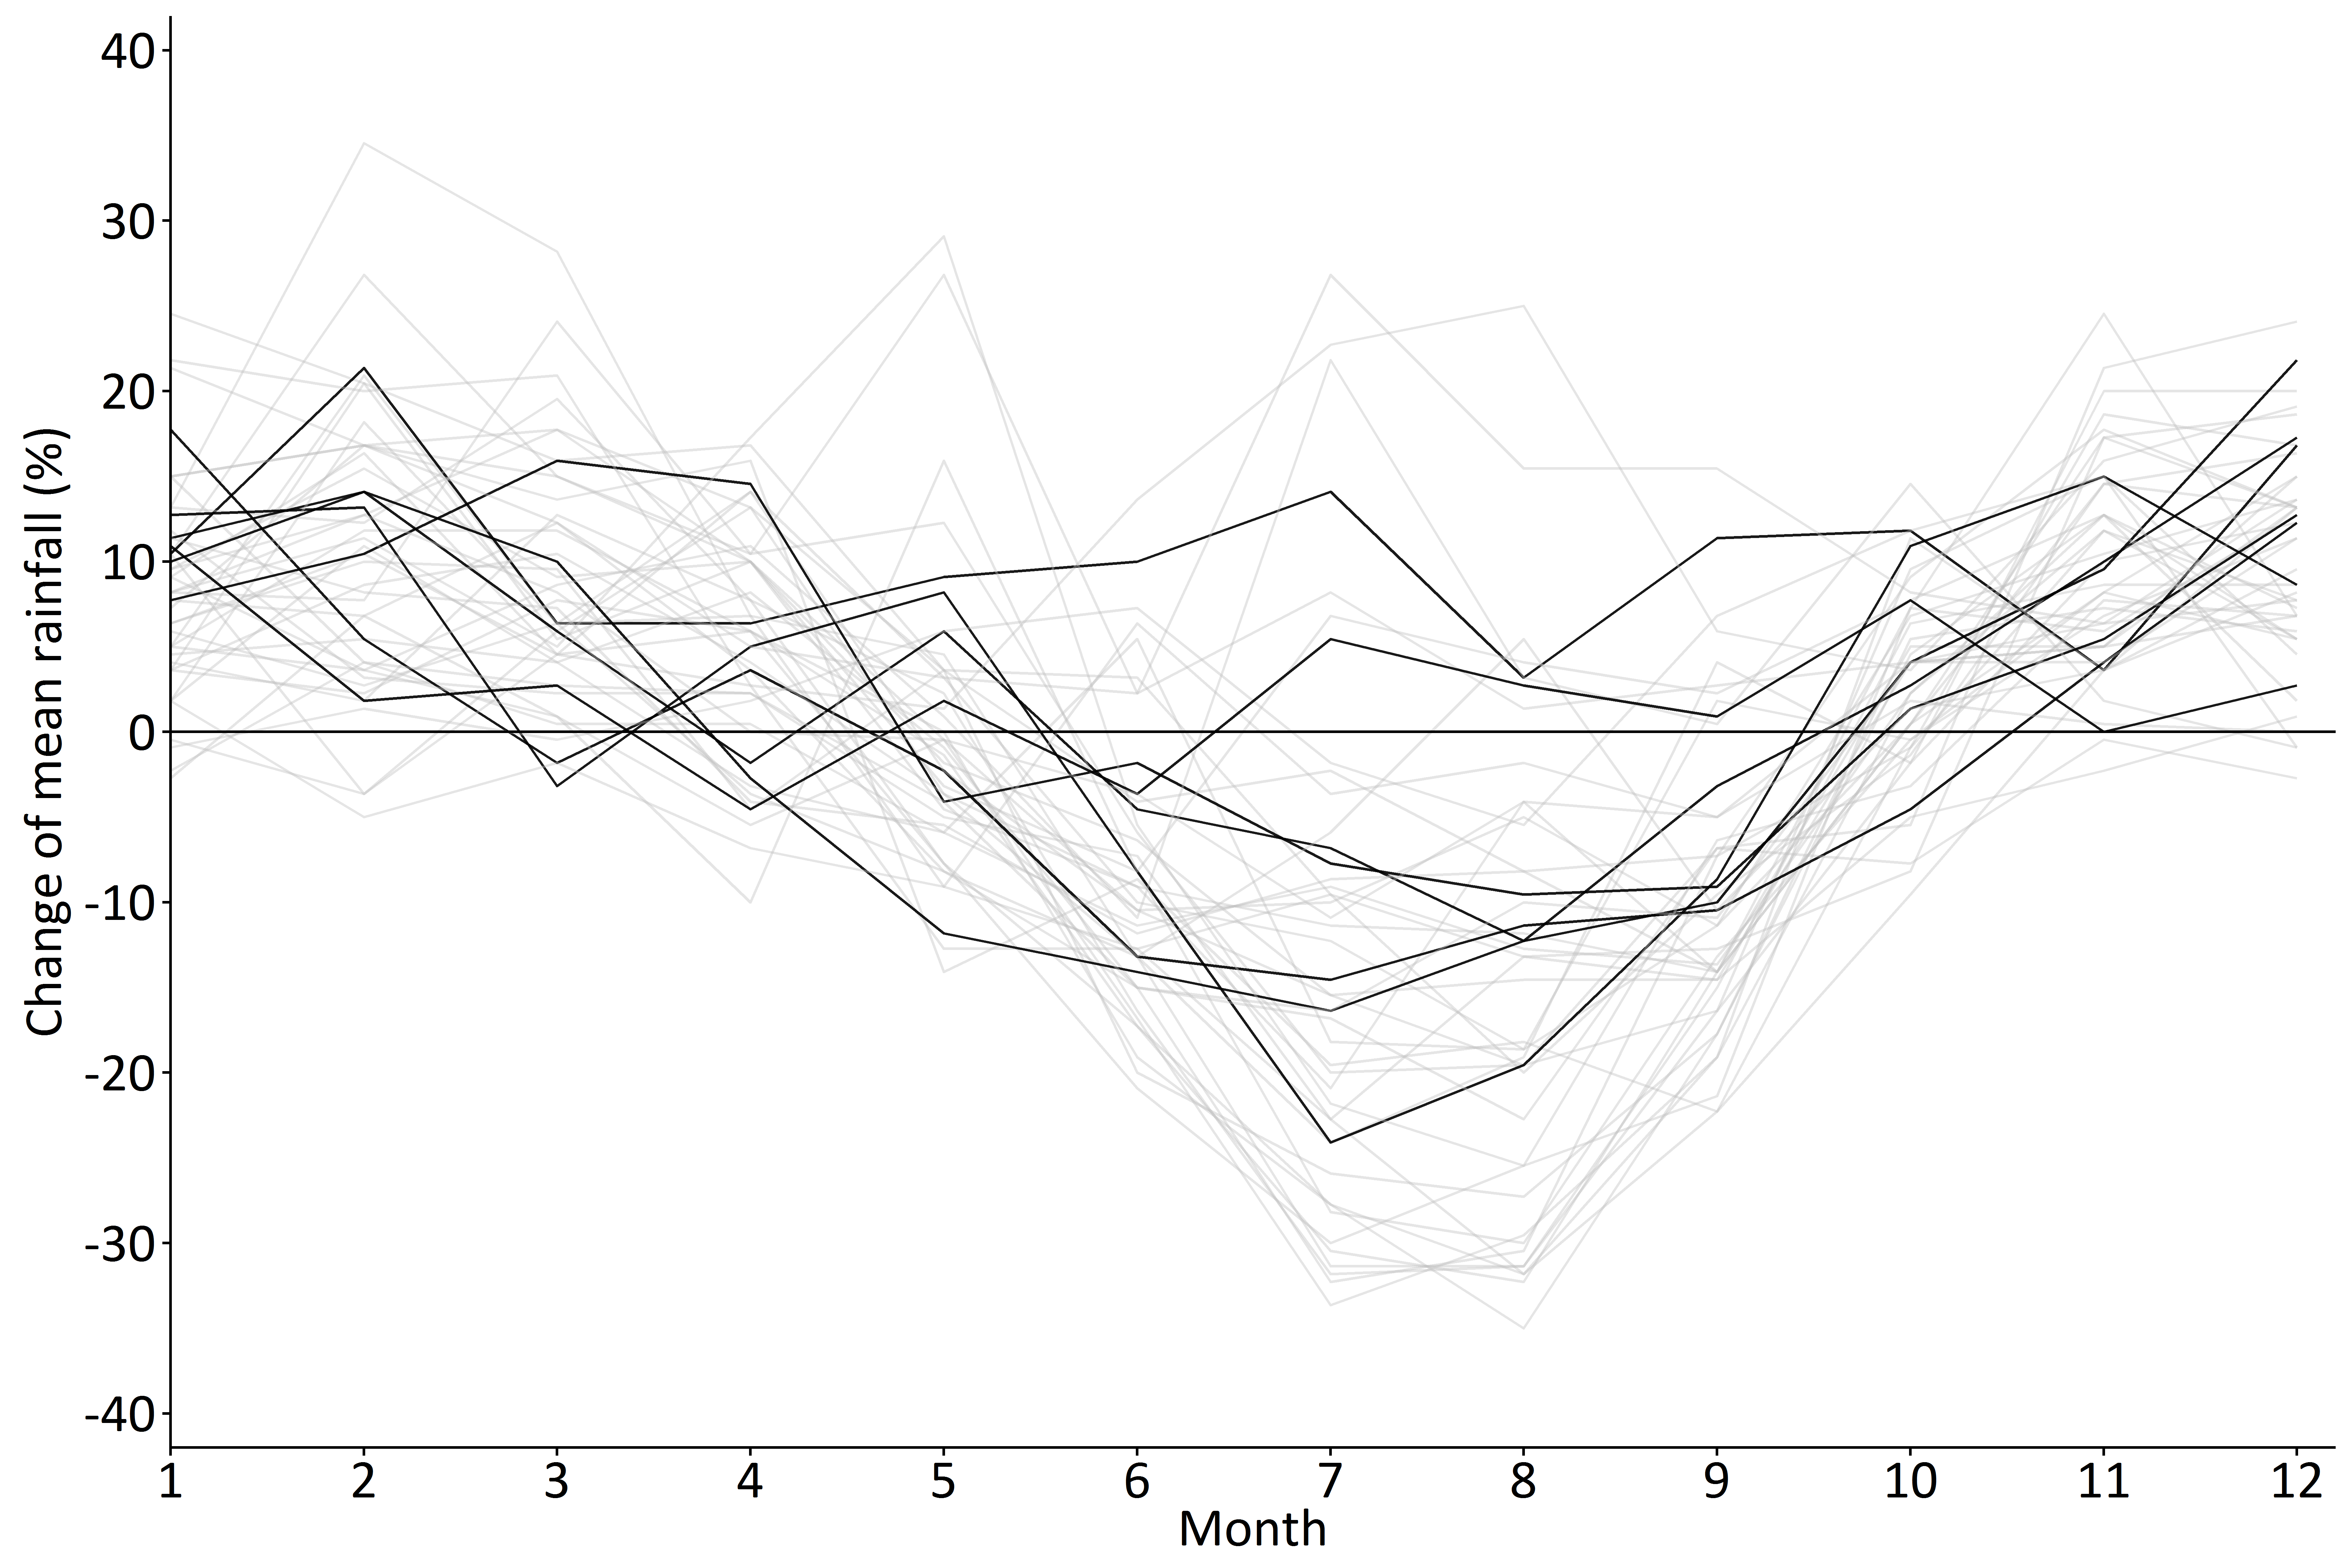
\includegraphics[width=\textwidth]{PerturbRain.png}
		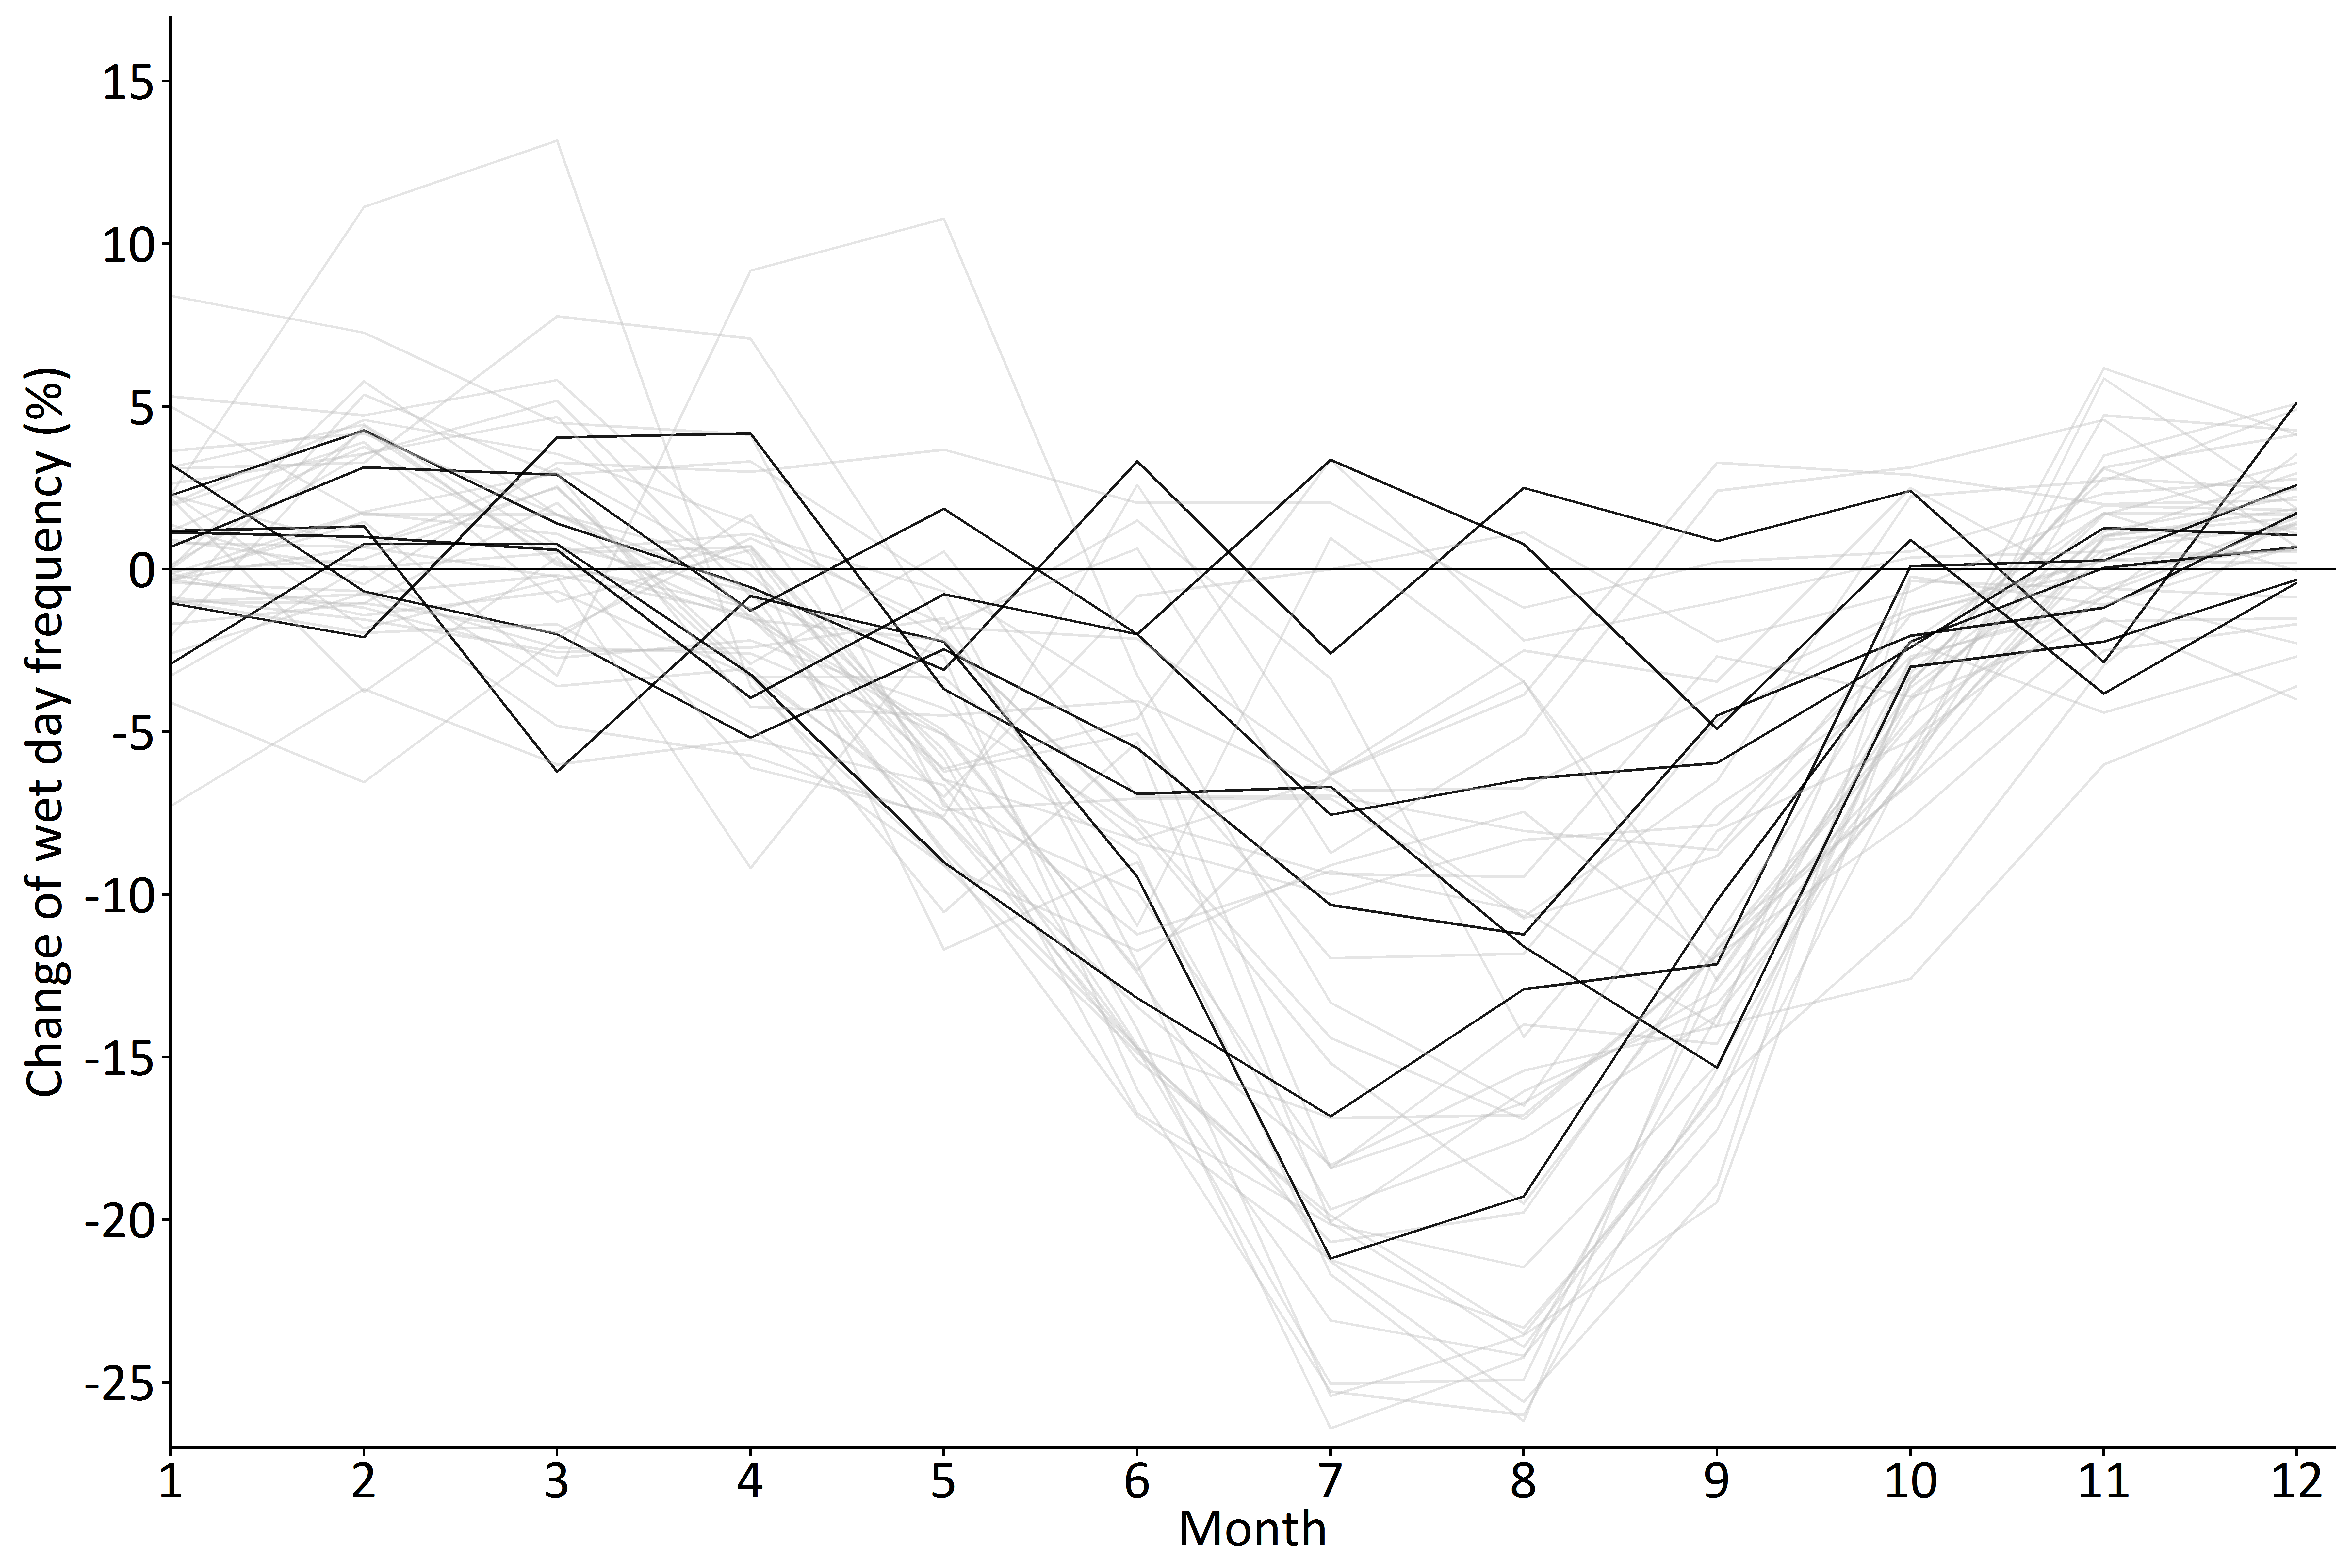
\includegraphics[width=\textwidth]{PerturbRainfreq.png}
	\caption{Relative change of mean monthly rainfall (top) and wet day frequency (bottom) in future climatic conditions (2050) as compared to historical conditions (2000) for RCP 8.5. Black lines present the climate signals selected for the climate model ensemble, while grey lines present the additional climate signals that were used to define the synthesized scenarios. A positive value represents an increase of rainfall, while a negative represents a decrease of  rainfall. }
	\label{fig:AppB_PerturbRain}
\end{figure} 

\begin{figure}[tbhp]
	\centering
		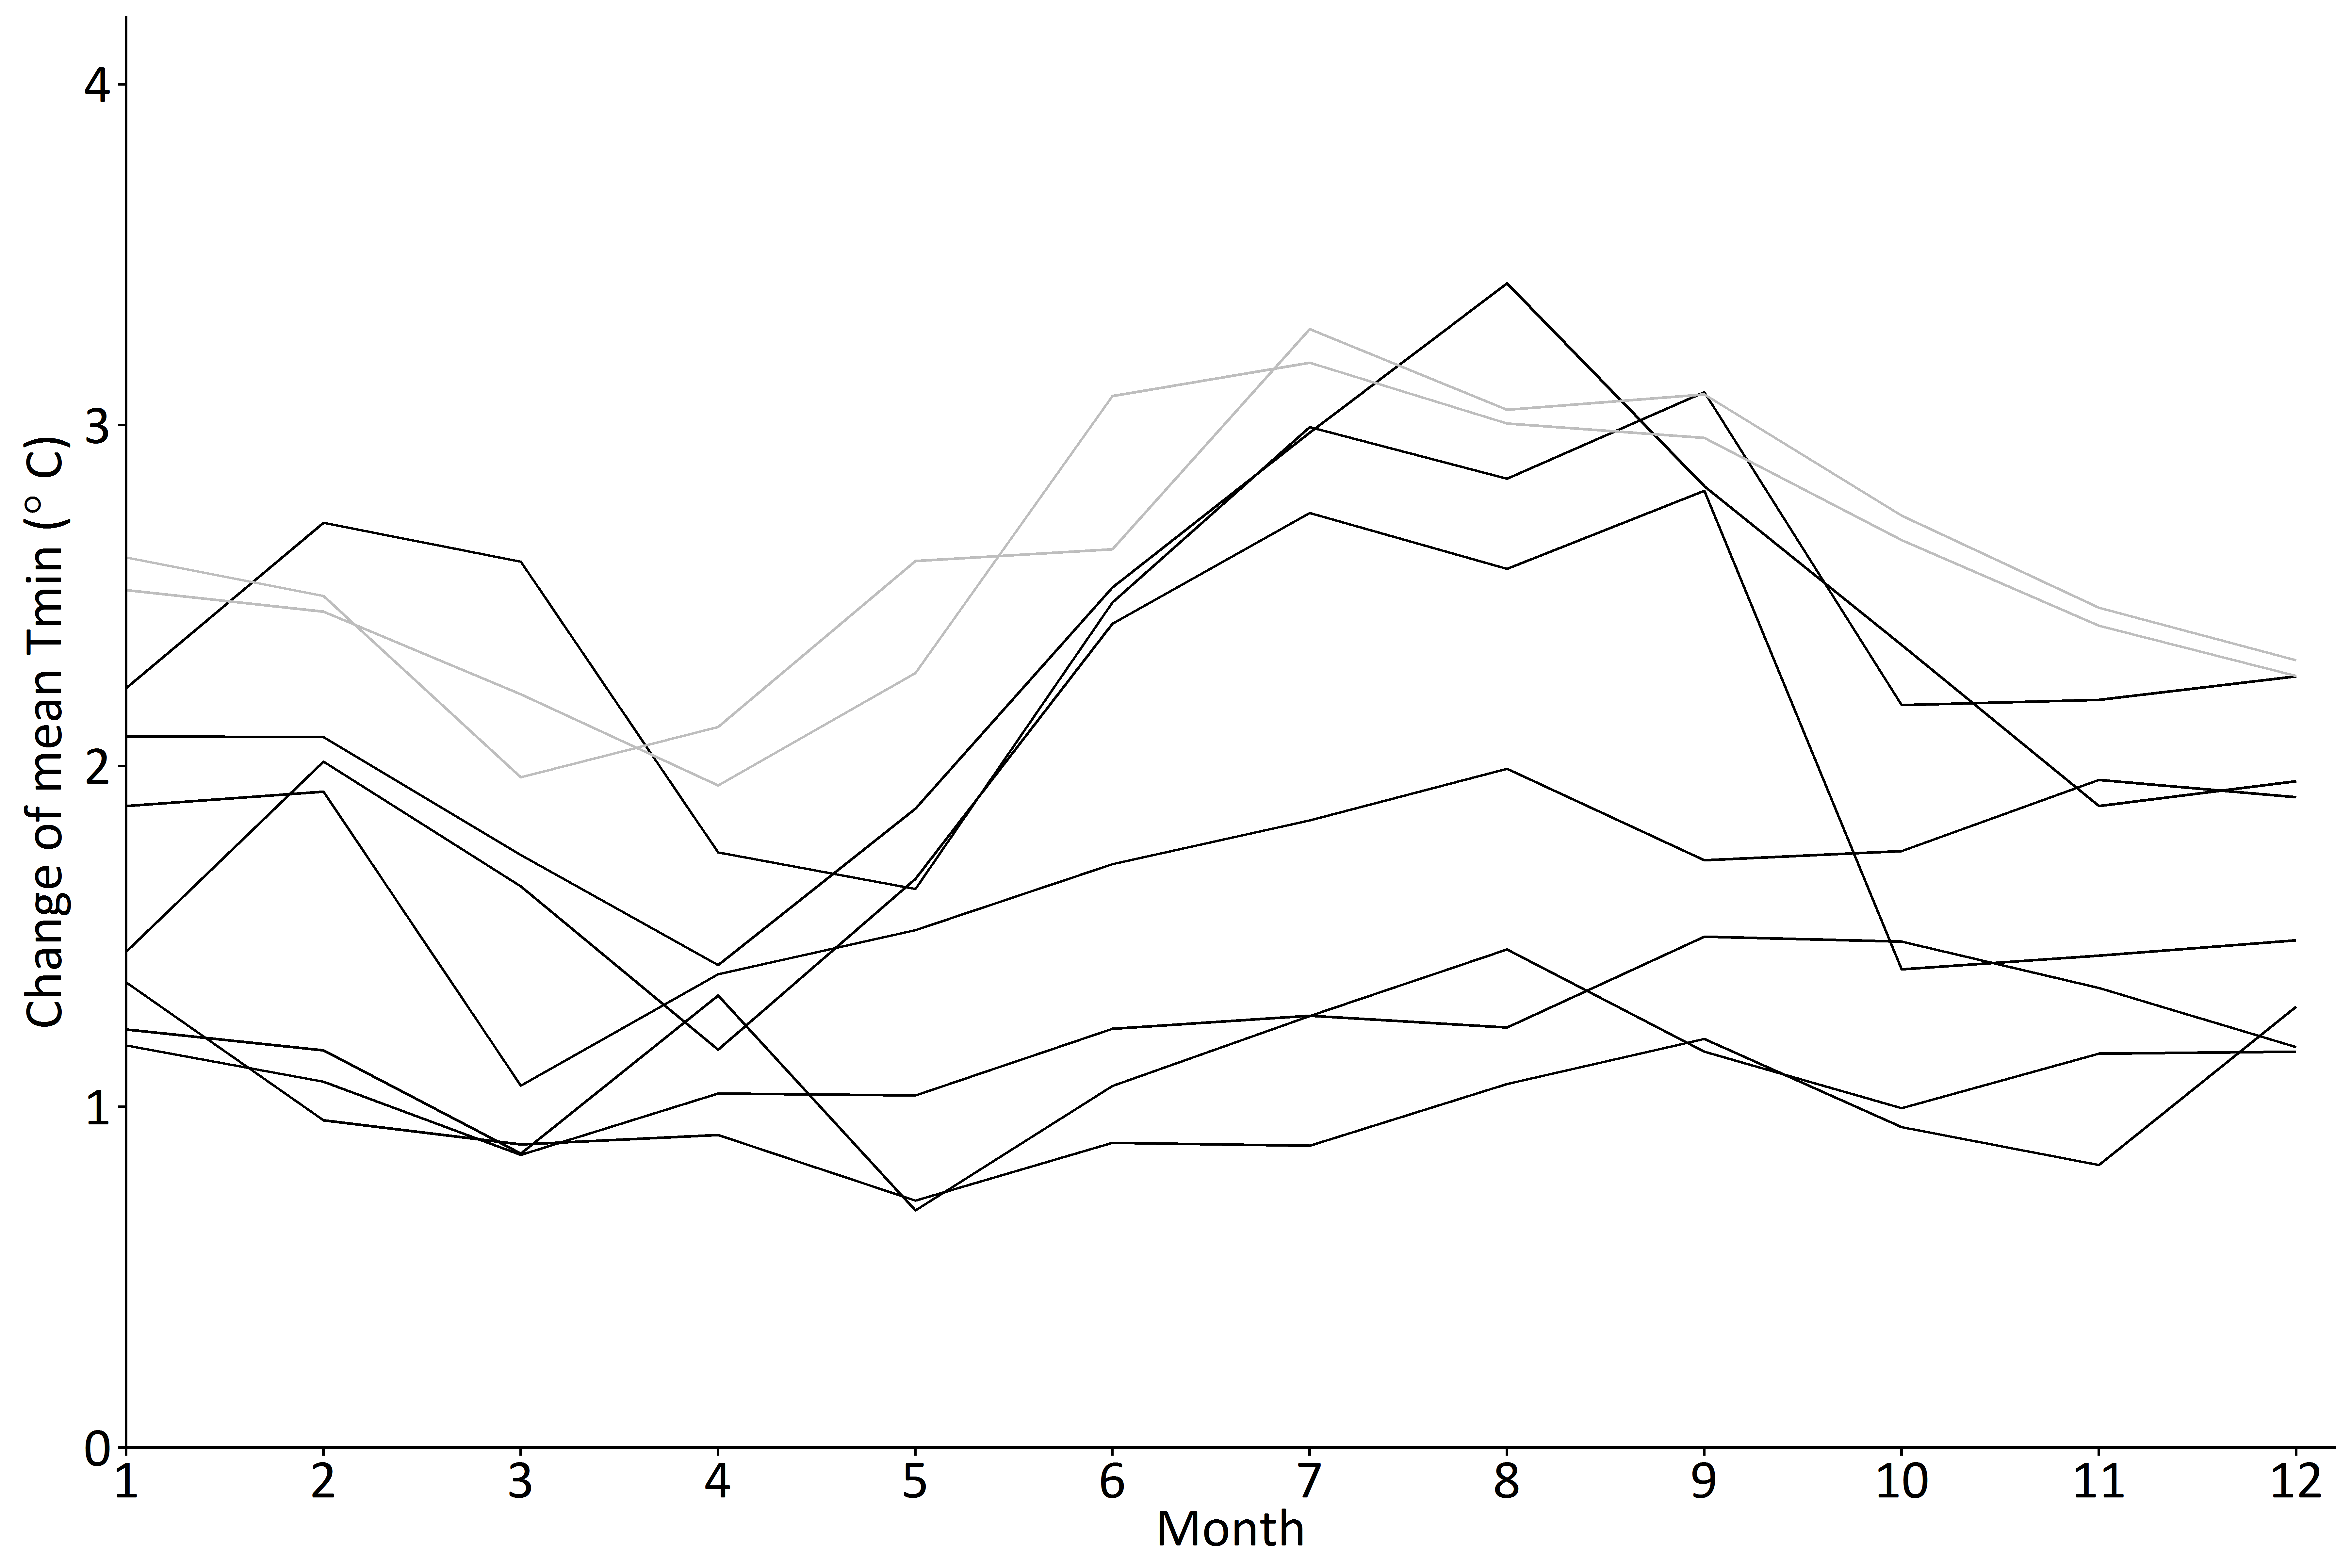
\includegraphics[width=\textwidth]{PerturbTmin.png}
		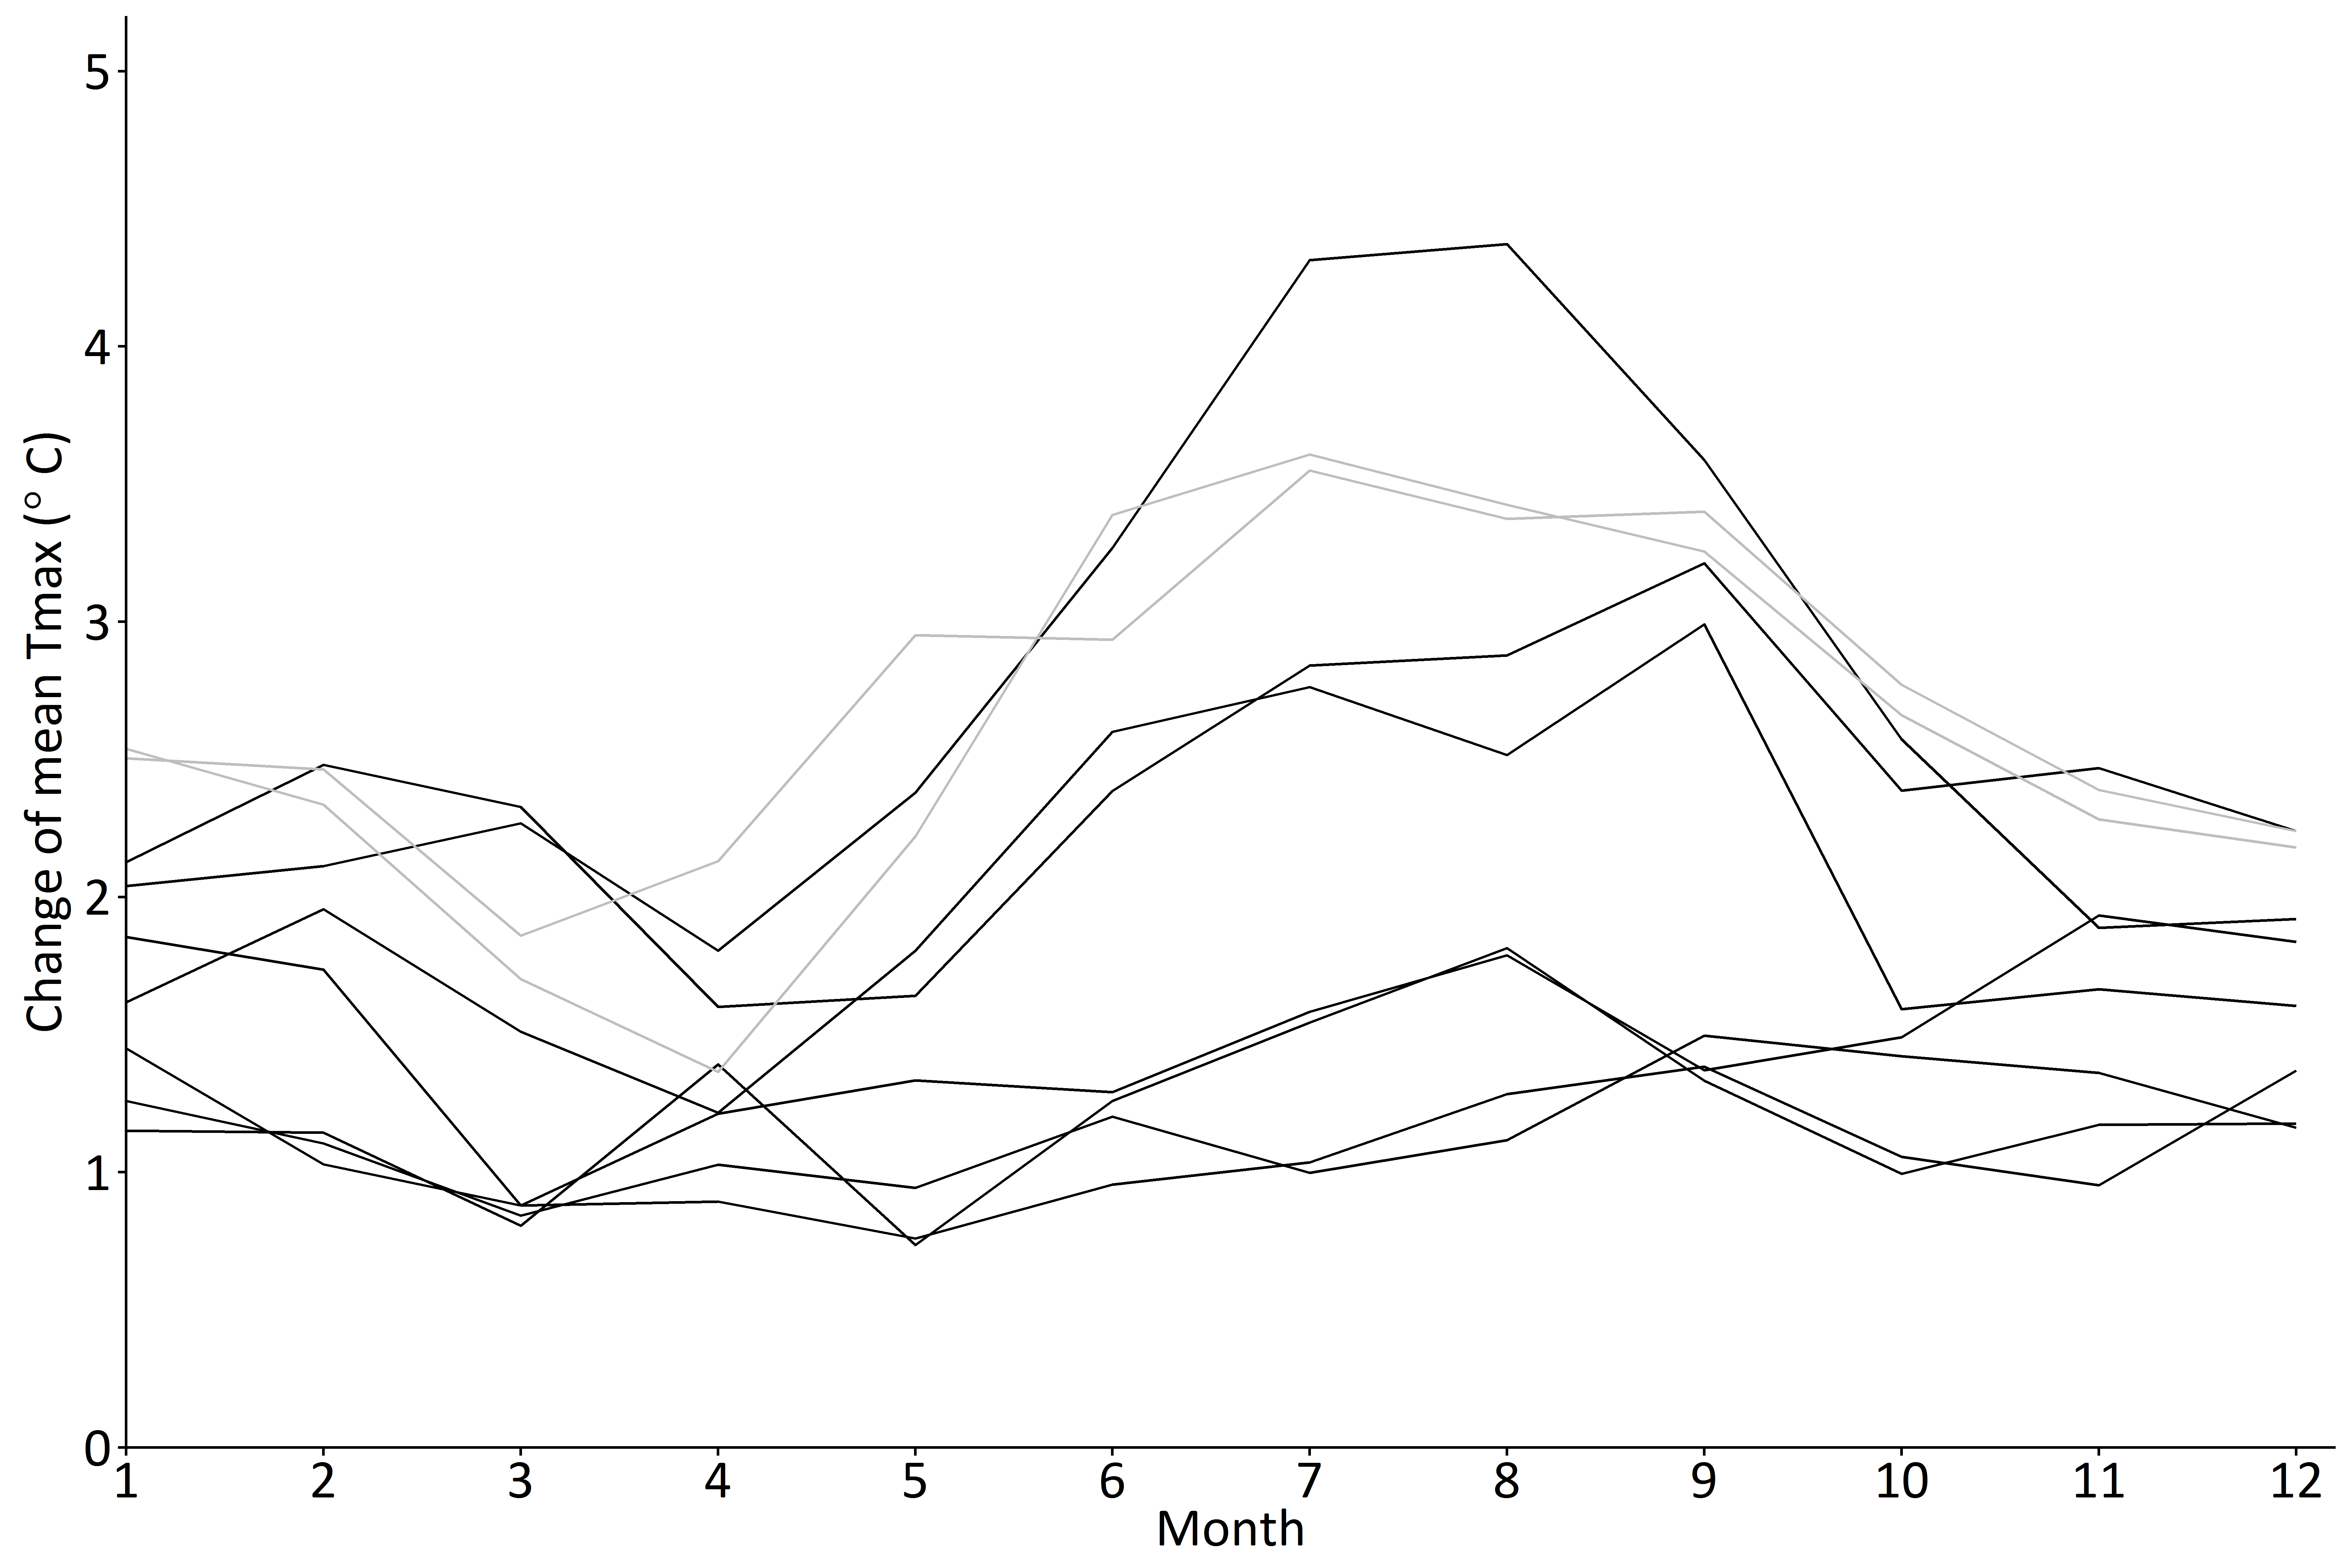
\includegraphics[width=\textwidth]{PerturbTmax.png}
	\caption{ Absolute change of mean monthly minimum temperature(\Tmin, top) and maximum temperature (\Tmax, bottom) in future climatic conditions (2050) as compared to historical conditions (2000) for RCP 8.5. Black lines present the climate signals selected for the climate model ensemble, while grey lines present the additional climate signals that were used to define the synthesized scenarios. A positive value represents a temperature increase, while a negative value represents a temperature decrease.}
	\label{fig:AppB_PerturbTemp}
\end{figure} 

\begin{footnotesize}
\begin{landscape}
\begin{tabularx}{\linewidth}{lp{2.3cm}XXXXXXXXXX}
\caption{Crop parameter for all simulated crops in the Plankbeek catchment, Flanders, Belgium.}\\
\toprule
Parameter & Units & Winter Wheat & Winter Barley & Maize & Sugar beet & Potato & Peas  & Carrot & Green beans & Grassland & Decidious forest \\
\midrule
\endfirsthead

\caption*{\autoref{tab:AnB_croppar} Cont.:Crop parameter for all simulated crops in the Plankbeek catchment, Flanders, Belgium.}\\
\toprule
Parameter & Units & Winter Wheat & Winter Barley & Maize & Sugar beet & Potato & Peas  & Carrot & Green beans & Grassland & Decidious forest \\
\midrule
\endhead

typ   &       & 2     & 2     & 2     & 3     & 3     & 2     & 3     & 2     & 1     & 1 \\
sow   &       & 1     & 1     & 1     & 1     & 0     & 1     & 1     & 1     & 1     & 1 \\
m     &       & 0     & 0     & 0     & 0     & 0     & 0     & 0     & 0     & 1     & 1 \\
tb    & °C    & 2     & 0     & 8     & 5     & 2     & 0     & 2     & 6     & 2     & 10 \\
tup   & °C    & 26    & 15    & 30    & 30    & 26    & 30    & 26    & 30    & 40    & 30 \\
pexup &       & 0.2   & 0.2   & 0.14  & 0.2   & 0.2   & 0.1   & 0.1   & 0.05  & 0.2   & 0.2 \\
pexlw &       & 0.65  & 0.65  & 0.72  & 0.6   & 0.6   & 0.45  & 0.45  & 0.55  & 0.55  & 0.55 \\
pexshp &       & 5     & 3     & 2.9   & 3     & 3     & 3     & 3     & 3     & 3     & 3 \\
psto  &       & 0.65  & 0.6   & 0.69  & 0.65  & 0.55  & 0.45  & 0.35  & 0.4   & 0.55  & 0.5 \\
pstoshp &       & 2.5   & 3     & 6     & 3     & 3     & 3     & 3     & 3     & 3     & 3 \\
psen  &       & 0.7   & 0.55  & 0.69  & 0.75  & 0.7   & 0.45  & 0.45  & 0.7   & 0.85  & 0.85 \\
psenshp &       & 2.5   & 3     & 2.7   & 3     & 3     & 3     & 3     & 3     & 3     & 3 \\
etos  & mm    & 0     & 0     & 0     & 0     & 0     & 0     & 0     & 0     & 0     & 0 \\
ppol  &       & 0.85  & 0.85  & 0.8   & 0.8   & 0.8   & 0.76  & 0.8   & 0.92  & 0.9   & 0.9 \\
anaer & vol\% below \Tsat & 5     & 15    & 5     & 5     & 5     & 5     & 5     & 5     & 2     & 4 \\
polmn & °C    & 5     & 5     & 10    & 8     & -     & -     & -     & -     & 8     & 10 \\
polmx & °C    & 35    & 35    & 40    & 40    & -     & -     & -     & -     & 40    & 40 \\
stbio & °C/day & 8     & 8     & 13    & 9     & 8     & 14    & 8     & 14    & 13    & - \\
kc    &       & 1.1   & 1.1   & 1.05  & 1.1   & 1.1   & 1.1   & 0.95  & 1.1   & 0.85  & 0.95 \\
kcdcl & \%/day & 0.15  & 0.15  & 0.3   & 0.15  & 0.15  & 0.15  & 0.15  & 0.15  & 0.15  & 0.15 \\
rtn   & m     & 0.3   & 0.3   & 0.3   & 0.3   & 0.3   & 0.3   & 0.3   & 0.3   & 0.3   & 1.5 \\
rtx   & m     & 1.5   & 1.3   & 1.1   & 1     & 0.6   & 0.5   & 0.6   & 0.6   & 0.6   & 1.5 \\
rtshp &       & 15    & 15    & 13    & 15    & 15    & 15    & 15    & 15    & 15    & 13 \\
rtexup & m3/m3 soil/day & 0.028 & 0.019 & 0.021 & 0.025 & 0.088 & 0.048 & 0.088 & 0.04  & 0.04  & 0.016 \\
rtexlw & m3/m3 soil/day & 0.008 & 0.006 & 0.007 & 0.006 & 0.022 & 0.012 & 0.022 & 0.01  & 0.01  & 0.004 \\
evardc &       & 50    & 50    & 50    & 60    & 60    & 60    & 60    & 60    & 60    & 60 \\
ccs   & cm2   & 0.75  & 0.75  & 6.5   & 1     & 20    & 4.05  & 0.5   & 5     & 5     & 5 \\
den   & plants/ha & 2000000 & 2000000 & 75000 & 100000 & 32000 & 810000 & 1000000 & 300000 & 300000 & 100000 \\
\CCx   & m2/m2 & 0.92  & 0.92  & 0.87  & 0.98  & 1     & 0.9   & 0.95  & 1     & 0.9   & 0.9 \\
det   &       & 1     & 1     & 1     & 0     & 0     & 0     & 0     & 0     & 0     & 0 \\
exc   & \%    & 100   & 100   & 50    & -     & -     & 20    & -     & 100   & 20    & 20 \\
\WPster  & g/m2  & 18.5  & 18.5  & 33.7  & 17    & 18.5  & 14    & 18.5  & 15    & 17    & 17 \\
fwpy  & \%    & 100   & 100   & 100   & 100   & 100   & 100   & 100   & 100   & 100   & 100 \\
fsink & \%    & 0     & 0     & 0     & 50    & 75    & 60    & 60    & 60    & 50    & 50 \\
hio   & \%    & 52    & 33    & 52    & 70    & 90    & 34    & 60    & 22    & -     & - \\
hipsflo & \%    & 5     & 5     & 0     & 0     & 2     & -     & 2     & 2     & -     & - \\
hipsveg &       & 10    & 10    & 7     & 4     & -     & 4     & -     & 0.5   & -     & - \\
hingsto &       & 7     & 5     & 3     & -     & 10    & 3     & 10    & 10    & -     & - \\
hinc  & \%    & 15    & 15    & 15    & 20    & 5     & 0     & 5     & 60    & -     & - \\
eme   & GDD or day & 100   & 100   & 50    & 20    & 150   & 30    & 67    & 110   & 0     & 0 \\
root  & GDD or day & 1200  & 1200  & 1200  & 617   & 650   & 478   & 488   & 650   & 31    & 26 \\
sen   & GDD or day & 1550  & 1550  & 1100  & 1450  & 1550  & 864   & 1603  & 850   & 170   & 174 \\
mat   & GDD or day & 1900  & 1900  & 1200  & 1850  & 1850  & 945   & 1850  & 870   & 215   & 205 \\
flo   & GDD or day & 1200  & 1200  & 650   & 650   & 650   & 302   & 488   & 450   & 0     & 0 \\
flolen & GDD or day & 180   & 180   & 180   & 0     & 0     & 300   & 0     & 300   & 0     & 0 \\
cgc   & m2/m2/GDD or m2/m2/day & 0.008 & 0.008 & 0.012 & 0.012 & 0.009 & 0.014 & 0.01  & 0.014 & 0.214 & 0.164 \\
cdc   & m2/m2/GDD or m2/m2/day & 0.008 & 0.008 & 0.01  & 0.004 & 0.008 & 0.002 & 0.004 & 0.002 & 0.045 & 0.086 \\
hilen & GDD or day & 550   & 550   & 500   & 1100  & 1100  & 566   & 1267  & 400   & -     & - \\
\bottomrule
  \label{tab:AnB_croppar}%
\end{tabularx}
\end{landscape}


\begin{tabularx}{\textwidth}{lccccc}
\caption{Changes in seasonal crop yield, crop water productivity (\WPET), length of the growing period (LGP), water stress index (WSI) and cold stress index (CSI) in 2050 under traditional management as compared to historical conditions (1985-2014) for the Plankbeek catchment (n=30). Presented ranges for future conditions represent the variety between the median values of the 7 GCMs. A positive change value represents an increase, while a negative value represents a decrease.}\\
\toprule
\multicolumn{1}{c}{\multirow{2}[1]{*}{\textbf{}}} & \multirow{2}[1]{*}{\textbf{}} & \multirow{2}[1]{*}{\textbf{Historical}} & \multicolumn{3}{c}{\textbf{Future median change}} \\
\multicolumn{1}{c}{} &       &  median     & \multicolumn{3}{c}{\textbf{under traditional management}} \\
\multicolumn{1}{l}{\textbf{}} & \textbf{} & \textbf{} & \textbf{minimum} & \textbf{median} & \textbf{maximum} \\
\midrule
\multicolumn{1}{l}{\textbf{Maize  }} &       &       &       &       &  \\
\multicolumn{1}{l}{Yield} & (t/ha) & 10.19 & -1.163 & +0.144 & +0.478 \\
\multicolumn{1}{l}{\WPET} & (kg/m3) & 2.64  & +0.10 & +0.29 & +0.35 \\
\multicolumn{1}{l}{LGP} & (days) & 133   & -33   & -22   & -14 \\
\multicolumn{1}{l}{WSI} & \%    & 4.1   & -0.9  & -0.2  & +6.8 \\
\multicolumn{1}{l}{CSI} & \%    & 30.5  & -15.5 & -10.5 & -7.0 \\
\midrule
\multicolumn{1}{l}{\textbf{Winter wheat }} &       &       &       &       &  \\
\multicolumn{1}{l}{Yield} & (t/ha) & 11.291 & +2.309 & +2.400 & +2.755 \\
\multicolumn{1}{l}{\WPET} & (kg/m3) & 2.46  & +1.01 & +1.10 & +1.57 \\
\multicolumn{1}{l}{LGP} & (days) & 251   & -30   & -22   & -15 \\
\multicolumn{1}{l}{WSI} & \%    & 0.0   & 0.0   & 0.0   & 0.0 \\
\multicolumn{1}{l}{CSI} & \%    & 33.0  & -11.0 & -8.0  & -5.0 \\
\midrule
\multicolumn{1}{l}{\textbf{Potato }} &       &       &       &       &  \\
\multicolumn{1}{l}{Yield} & (t/ha) & 11.388 & -0.830 & +1.375 & +2.826 \\
\multicolumn{1}{l}{\WPET} & (kg/m3) & 3.35  & +0.28 & +0.91 & +1.24 \\
\multicolumn{1}{l}{LGP} & (days) & 116   & -19   & -11   & -7 \\
\multicolumn{1}{l}{WSI} & \%    & 16.6  & -1.5  & +3.6  & +15.7 \\
\multicolumn{1}{l}{CSI} & \%    & 0.0   & 0.0   & 0.0   & 0.0 \\
\midrule
\multicolumn{1}{l}{\textbf{Sugar beet }} &       &       &       &       &  \\
\multicolumn{1}{l}{Yield} & (t/ha) & 14.061 & -1.668 & +0.948 & +1.980 \\
\multicolumn{1}{l}{\WPET} & (kg/m3) & 3.16  & +0.02 & +0.43 & +0.75 \\
\multicolumn{1}{l}{LGP} & (days) & 168   & -38   & -25   & -17 \\
\multicolumn{1}{l}{WSI} & \%    & 3.1   & -1.0  & 1.5   & 12.1 \\
\multicolumn{1}{l}{CSI} & \%    & 6.5   & -3.5  & -3.5  & -2.5 \\
\midrule
\multicolumn{1}{l}{\textbf{Peas}} &       &       &       &       &  \\
\multicolumn{1}{l}{Yield} & (t/ha) & 2.096 & +0.264 & +0.456 & +0.558 \\
\multicolumn{1}{l}{\WPET} & (kg/m3) & 1.09  & +0.30 & +0.37 & +0.41 \\
\multicolumn{1}{l}{LGP} & (days) & 73    & -7    & -6    & -4 \\
\multicolumn{1}{l}{WSI} & \%    & 15.4  & -1.3  & -0.1  & 5.1 \\
\multicolumn{1}{l}{CSI} & \%    & 14.0  & -6.0  & -4.0  & -3.0 \\
\bottomrule
  \label{tab:AnB_ChangeTradMan}%
\end{tabularx}%
\clearpage


\begin{tabularx}{\textwidth}{lccccc}
\caption{Changes in seasonal crop yield, crop water productivity (\WPET), length of the growing period (LGP), water stress index (WSI) and cold stress index (CSI) in 2050 under adapted management as compared to historical conditions (1985-2014) for the Plankbeek catchment (n=30). Presented ranges for future conditions represent the variety between the median values of the 7 GCMs. A positive change value represents an increase, while a negative value represents a decrease.}\\
\toprule
\multicolumn{1}{c}{\multirow{2}[1]{*}{\textbf{}}} & \multirow{2}[1]{*}{\textbf{}} & \multirow{2}[1]{*}{\textbf{Historical}} & \multicolumn{3}{c}{\textbf{Future median change}} \\
\multicolumn{1}{c}{} &       &  median     & \multicolumn{3}{c}{\textbf{under adapted management}} \\
\multicolumn{1}{l}{\textbf{}} & \textbf{} & \textbf{} & \textbf{minimum} & \textbf{median} & \textbf{maximum} \\
\midrule
\textbf{Maize  } &       &       &       &       &  \\
Yield & (t/ha) & 10.19 & +0.563 & +1.567 & +1.982 \\
WPET  & (kg/m³) & 2.64  & +0.35 & +0.62 & +0.64 \\
LGP   & (days) & 133   & -22   & -8    & +1 \\
WSI   & \%    & 4.1   & -1.9  & -1.1  & +2.7 \\
CSI   & \%    & 30.5  & -15.1 & -9.5  & -6.5 \\
\midrule
\textbf{Winter wheat } &       &       &       &       &  \\
Yield & (t/ha) & 11.291 & +2.911 & +3.069 & +3.428 \\
WPET  & (kg/m³) & 2.46  & +0.98 & +1.12 & +1.55 \\
LGP   & (days) & 251   & -24   & -16   & -10 \\
WSI   & \%    & 0.0   & 0.0   & 0.0   & 0.0 \\
CSI   & \%    & 33.0  & -11.0 & -8.0  & -6.0 \\
\midrule
\textbf{Potato } &       &       &       &       &  \\
Yield & (t/ha) & 11.388 & -0.180 & +1.920 & +3.638 \\
WPET  & (kg/m³) & 3.35  & +0.38 & +0.96 & +1.23 \\
LGP   & (days) & 116   & -15   & -7    & -4 \\
WSI   & \%    & 16.6  & -4.0  & +2.6  & +14.2 \\
CSI   & \%    & 0.0   & 0.0   & 0.0   & 0.0 \\
\midrule
\textbf{Sugar beet } &       &       &       &       &  \\
Yield & (t/ha) & 14.061 & -0.469 & +2.906 & +4.030 \\
WPET  & (kg/m³) & 3.16  & +0.21 & +0.72 & +1.07 \\
LGP   & (days) & 168   & -23   & -9    & +0 \\
WSI   & \%    & 3.1   & -1.0  & +2.7  & +12.7 \\
CSI   & \%    & 6.5   & -2.5  & -1.5  & +0.0 \\
\midrule
\textbf{Peas} &       &       &       &       &  \\
Yield & (t/ha) & 2.096 & +0.564 & +0.747 & +0.833 \\
WPET  & (kg/m³) & 1.09  & +0.42 & +0.50 & +0.55 \\
LGP   & (days) & 73    & -3    & +0    & +3 \\
WSI   & \%    & 15.4  & -3.7  & -2.8  & +1.7 \\
CSI   & \%    & 14.0  & -4.0  & -3.0  & -2.0 \\
\bottomrule
  \label{tab:AnB_ChangeAdapMan}%
\end{tabularx}%
\clearpage

\begin{tabularx}{\textwidth}{lcccc}
\caption{Changes in median annual discharge in 2050 as compared to historical conditions (1985-2014) for the Plankbeek catchment under traditional and adapted management (n=30). Presented ranges (minimum, median and maximum) for future conditions represent the variety between the median values of the 7 GCMs. A positive change value represents an increase, while a negative value represents a decrease of flow.}\\
\toprule
\multicolumn{1}{c}{\multirow{2}[1]{*}{\textbf{}}} & \textbf{Historical} & \multicolumn{3}{c}{\multirow{2}[1]{*}{\textbf{Future median change (\%)}}} \\
\multicolumn{1}{c}{} & \textbf{ median} & \multicolumn{3}{c}{} \\
\multicolumn{1}{l}{\textbf{}} & \textbf{(mm/year)} & \textbf{minimum} & \textbf{median} & \textbf{maximum} \\
\midrule
\textbf{Traditional management} &       &       &       &  \\
Annual total discharge & 277   & +11   & +31   & +77 \\
Annual baseflow & 157   & -1    & +10   & +44 \\
Annual interflow & 43    & -3    & +3    & +12 \\
Annual overland flow & 77    & +6    & +10   & +20 \\
\midrule
\textbf{Adapted management} &       &       &       &  \\
Annual total discharge & 277   & +10   & +28   & +75 \\
Annual baseflow & 157   & +11   & +23   & +59 \\
Annual interflow & 43    & 0     & +5    & +14 \\
Annual overland flow & 77    & -9    & -6    & +2 \\
\bottomrule
  \label{tab:AnB_ChangeQ}%
\end{tabularx}%
\end{footnotesize}


\cleardoublepage
